\documentclass[../report.tex]{subfiles}
\begin{document}

\section*{\centering First Report}

\textbf{Group number:} 11 \\
\textbf{Authors:} Mathias Emil Slettmark-Nielsen(masle16) \& Mikkel Larsen(milar16)

\subsection*{Essential Behaviours to Complete the Sokoban Game}
%What behaviours or functions will you equip the robot with, so it can complete the Sokoban course successfully?

For the robot to move around the map some basic behaviours are needed. The map is made of lines, which the robot must follow. Therefore, a behaviour needed is to follow a line. Thus, making the robot able to stay on the map and obey the rules of the game. This behaviour will be a reactive controller behaviour, where the robot reacts when it is straying from the line. This means the color sensors are directly controlling the two large motors. 

To make the environment easy for the robot to interact with, the robot is only told to go from intersection to intersection. The idea is to create a sequence of simple tasks, which the robot solves one by one. The sequence is made by the sokoban solver and would consist of the tasks described in table \ref{tab:behaviours}. Thus, the robot needs to be able to detect an intersection. An intersection is detected if the two color sensors see a line at the same time, within some small time delay. 

\begin{table}[H]
\begin{tabular}{|c|c|c|}
\hline
Number & Name & Description \\ \hline
1 & Forward & Follow a line until the next intersection is reached. \\ \hline
2 & Reverse & Reverse along a line until the next intersection is reached. \\ \hline
3 & Turn left & \begin{tabular}[c]{@{}c@{}}Rotate left until the left line of the intersection is \\ reached and then go forward (1).\end{tabular} \\ \hline
4 & Turn right & \begin{tabular}[c]{@{}c@{}}Rotate right until the right line of the intersection is \\ reached, and then go forward (1).\end{tabular} \\ \hline
4 & \begin{tabular}[c]{@{}c@{}} Rotate 180 \\ degrees \end{tabular} & \begin{tabular}[c]{@{}c@{}}Perform two right turns (4) in a row, except that the \\ first turn must not be followed by a forward.\end{tabular} \\ \hline
\end{tabular}
\caption{Behaviours for the robot to solve the sokoban puzzle.}
\label{tab:behaviours}
\end{table}

Table \ref{tab:behaviours} shows the behaviours the robot must have to solve the puzzle. 
The behaviours, follow a line and detect intersections are the most fundamental behaviors of the robot, which are crucial to make the robot stay on the map and make the robot aware of where it is. The behaviors in table \ref{tab:behaviours} is on the next behaviour layer and are used to navigate when an intersection is detected. 

A behaviour to navigate towards the can and check if the can is present in front of the robot is needed. Thus, the robot is able to drive more carefully when pushing a can.

\subsection*{Construction of the Robot Design}
%What implications do the choices in (1) have for the physical structure of the robot?  What sensors will you deploy, and where?  etc.

A sketch of the robot design, with the implemented components, is illustrated in figure \ref{fig:robot_design_sketch}. The following components are implemented on the robot: a LEGO Mindstorms EV3 kit, two large motors, two color sensors, a gyro sensor, and a sonar sensor. The large motors are implemented to make the robot move around the map. The color sensors enable the robot to detect lines. The gyro sensor helps the robot turn left, right or 180 degrees. The sonar sensor will make the robot able to detect when a can is in front of the robot. Each component is labeled on the sketch.

\begin{figure}[H]
    \centering
    \begin{subfigure}[b]{0.5\textwidth}
        \centering
        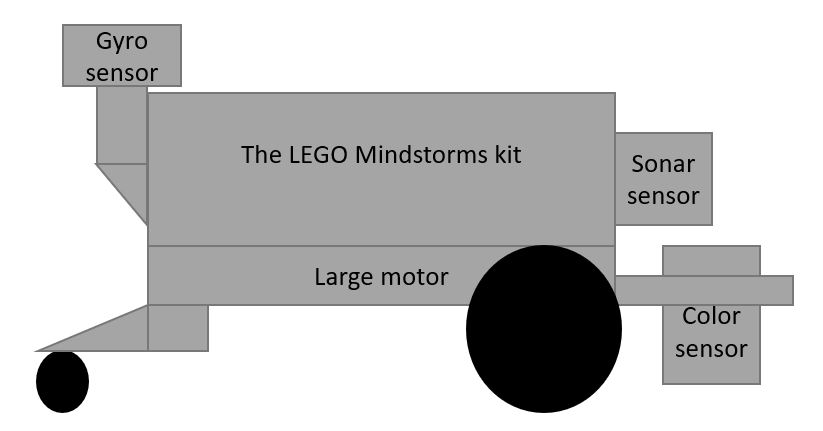
\includegraphics[width=\textwidth]{figures/robot_design/sketch_side_view.jpg}
        \caption{Side view of the robot design.}
        \label{fig:sketch_side_view}
    \end{subfigure}%
    \begin{subfigure}[b]{0.5\textwidth}
        \centering
        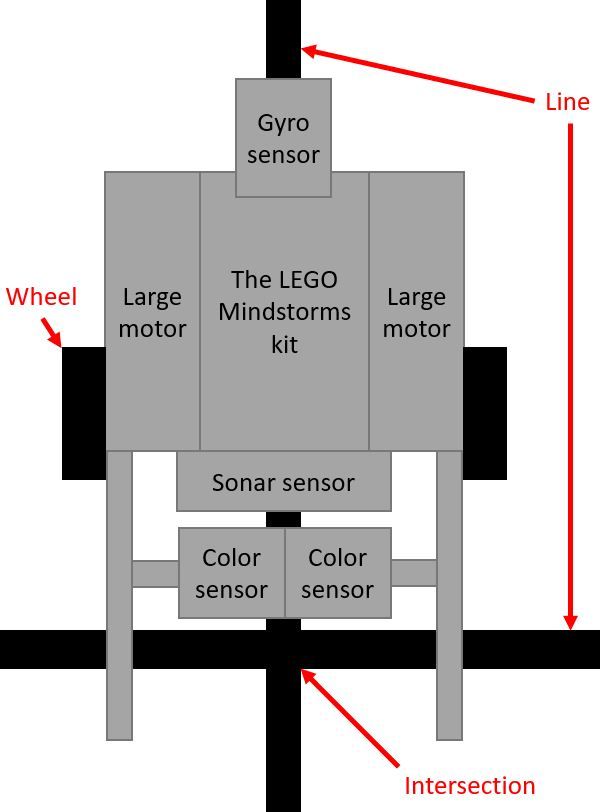
\includegraphics[width=0.65\textwidth]{figures/robot_design/sketch_top_view.jpg}
        \caption{Top view of the robot design.}
        \label{fig:sketch_top_view}
    \end{subfigure}
    \caption{Sketch of the robot design.}
    \label{fig:robot_design_sketch}
\end{figure}

The color sensors are mounted at the front of the robot, in front of the wheels. Thus, the color sensors will detect if the robot is straying away from the line in advance, thereby making the robot drive more smoothly. Furthermore, the color sensors are placed as close as possible to each other. This makes the robot able to react fast, because a small stray away from the line will be detected. The gyro sensor is placed at the back of the robot. Thus, making it able to detect when the robot rotates. The sonar sensor is placed at the front of the robot to detect when a can is close.

\subsection*{Factors which Affect the Speed and Reliability of the Robot}
%What factors do you think will affect the speed and reliability with which your robot can execute the Sokoban solution?
% How will you evaluate and optimize them? (Or, will you optimize them, in fact?)

The mounted color sensors measure the reflected light, thus, the sun becomes a factor. The sensor does not detect the line when the sun is shining directly on the map. Thereby, the robot is unable to follow a line and detect intersections. This problem is handled in the environment first, by adding sunlight protection to the sensors. Secondly, a calibration of the inputs from the sensors, when it is sunny and not sunny, will be made in the software.

The acceleration and deceleration, as well as the top speed of the large motors when the robot is line following, has an impact of the time to complete a sokoban puzzle. Furthermore, the behaviours of completing a sequence of simple tasks are also having an impact. This is because the robot stops at each intersection and waits for the next task thereby slowing the movement of the robot. 

\subsection*{Documentation of the Robot's Performance}
%How will you test and document your robot's performance for the final report?

The robot's performance will be measured by first documenting each behaviour, by testing if the robot can follow a line, detect an intersection, turn right, turn left, rotate 180 degrees, go backward and detect a can. This will be done in both cloudy and sunny weather. To obtain an optimal speed the behaviour, follow a line, is tested at different speeds. The behaviour which detects an intersection will be implemented by measuring when both color sensors detect a line. Furthermore, a delay is added to make the detection more robust. The optimal delay time must be found. The robot's ability to contain a can will be tested to conclude whether a front gripper is necessary.

The sokoban solver will be tested on different sokoban map. Thus, showing which sokoban puzzles it can solve and which it can not solve.

Afterward, the combination of the sokoban solver and the robot is documented by completing a sokoban game.

\end{document}